\section{Communicating with the satelitte}

\begin{figure}
	\begin{center}
		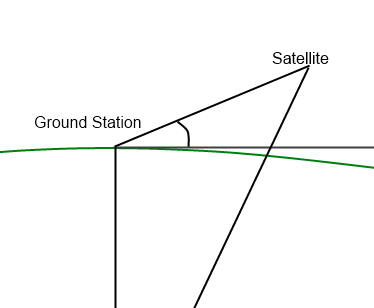
\includegraphics[width=0.7\textwidth]{Figures/groundstation_satelitte_geometry}
	\end{center}
\caption[Ground station satellite geometry]{Illustration of geometry between a ground station and a satelitte}
\label{fig:gs_s_geom}
\end{figure}

A ground station can only communicate with a satelitte when it has a certain elevation. This elevation can differ from case to case depending on atmospheric effects, frequency and more. 
In the following we assume that the minimum elevation is 25 degrees, maximum elevation is 90 degrees and no constraints on the azimuth angle.  For a illustration see Fig. \ref{fig:gs_s_geom}.


The result of this is that the ground station can communicate with the satelitte whenever the ground track is inside a rough circle centered on the ground station, see Fig. \ref{fig:ntnu_range} for the estimated "range" of the ground station at Gløshaugen with these constraints.

\begin{figure}
	\begin{center}
		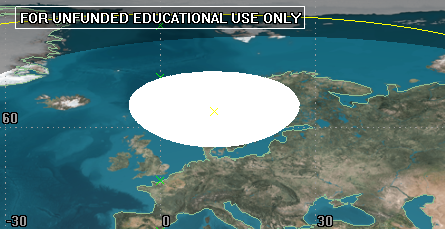
\includegraphics[width=0.8\textwidth]{Figures/ntnu_footprint}
	\end{center}
\caption[ntnu footprint]{NTNU ground station range}
\label{fig:ntnu_range}
\end{figure}